%% LyX 2.2.2 created this file.  For more info, see http://www.lyx.org/.
%% Do not edit unless you really know what you are doing.
\documentclass[english]{article}
\usepackage[T1]{fontenc}
\usepackage[latin9]{inputenc}
\usepackage{amsmath,amssymb,amsthm,latexsym,paralist,listings,graphicx}
\usepackage{geometry}
\geometry{verbose,tmargin=0.8in,bmargin=0.8in,lmargin=1in,rmargin=1in,headheight=0cm,headsep=0cm}
\usepackage{babel}
\usepackage[unicode=true]
 {hyperref}

\makeatletter

%%%%%%%%%%%%%%%%%%%%%%%%%%%%%% LyX specific LaTeX commands.
%% Because html converters don't know tabularnewline
\providecommand{\tabularnewline}{\\}

\makeatother

\begin{document}

\title{CSCE 221 Cover Page\\
 Homework Assignment \#2 \\
Due March 27 at 23:59 pm to eCampus}

\author{First Name~~Joseph~~Last Name ~~Martinsen~~~~UIN~~323006691~~}

\date{User Name ~~josephmart~~~~~~~E-mail address~~~josephmart@tamu.edu~~~~~~~~~\medskip{}
}
\maketitle
\begin{quotation}
Please list all sources in the table below including web pages which
you used to solve or implement the current homework. If you fail to
cite sources you can get a lower number of points or even zero, read
more Aggie Honor System Office \href{http://aggiehonor.tamu.edu/}{http://aggiehonor.tamu.edu/}\medskip{}
\medskip{}
\end{quotation}
\begin{tabular}{|c|c|c|c|}
\hline 
Type of sources  & ~~~AVL Tree Info~~~~~ & ~~~~~~~~~~~~~~~~~~~~~~~~ & ~~~~~~~~~~~~~~~~~~~~~~~\tabularnewline
 &  &  & \tabularnewline
\hline 
\hline 
People &  &  & \tabularnewline
 &  &  & \tabularnewline
\hline 
Web pages (provide URL)  & http://pages.cs.wisc.edu/ &  & \tabularnewline
 & ~ealexand/cs367/NOTES/AVL-Trees/index.html &  & \tabularnewline
\hline 
Printed material &  &  & \tabularnewline
 &  &  & \tabularnewline
\hline 
Other Sources  &  &  & \tabularnewline
 &  &  & \tabularnewline
\hline 
\end{tabular}

\date{\medskip{}
\medskip{}
}
\begin{quotation}
I certify that I have listed all the sources that I used to develop
the solutions/codes to the submitted work.

\textquotedblleft On my honor as an Aggie, I have neither given nor
received any unauthorized help on this academic work.\textquotedblright{} 
\end{quotation}

\date{\medskip{}
\medskip{}
}

\begin{tabular}{cccccc}
Your Name  & ~~~Joseph~~~~~~~ &  & ~~~~~~Martinsen~~~~~ & Date  & ~~~03/27/2017~~~~~~~\tabularnewline
\end{tabular}\newpage{}

\begin{center}
\textbf{Homework 2}
\par\end{center}

\begin{center}
\textbf{due March 27 at 11:59 pm to eCampus.}
\par\end{center}
\begin{enumerate}
\item (15 points) Write a recursive function that counts the number of nodes
in a singly linked list. Write a recurrence relation that represents
your algorithm. Solve the relation and obtain the running time of
the algorithm in Big-O.
\begin{enumerate}
  \item 
  \begin{lstlisting}[language=C++]
  int nodeCounter(Node* n)
  {
    if(temp = = nullptr) { return 0; }

    return nodeCounter(n->next()) + 1;
  }
  \end{lstlisting}
  
  \item
  nodeCounter$(0) = 0$ \\
  nodeCounter$(n) =$ nodeCounter$(n-1) + 1$ \\

  \item
  
  \begin{align*}
    T(n) \\
    T(n-1) \\
    T(n-2) \\
    \cdots \\
    T(0) \\
    0
  \end{align*}
  
  height of tree = nodeCounter$(n) = n$ \\
  The Big-$O: O(n)$
\end{enumerate}

\item (15 points) Write a recursive function that finds the maximum value
in an array of int values without using any loops. Write a recurrence
relation that represents your algorithm. Solve the relation and obtain
the running time of the algorithm in Big-O.
\begin{enumerate}
\item
  \begin{lstlisting}[language=C++]
int maxArray(int a[], int length)
{
    if (length == 1)
        return a[0];

    int maxNext = maxArray(a, length-1);

    if (a[length-1] > maxNext)
        return a[length-1];
    return maxNext;
}
  \end{lstlisting}
  
  \item
  maxArray$($array$, $size$) = maxArray$($array$, $size$-1) \\
  maxArray($array$, 1) =$ a[0]$ \\

  \item
  Solving the relation: maxArray($array$, 1) =$ a[n]$ \\
  The Big-$O: O(n)$
\end{enumerate}


\item (10 points) What data structure is most suitable to determine if a
string s is a palindrome, that is, it is equal to its reverse. For
example, \textquotedblleft racecar\textquotedblright{} and \textquotedblleft gohan
gasalamiimalasagnahog\textquotedblright{} are palindromes. Justify
your answer. Use Big-O notation to represent the efficiency of your
algorithm. \\ \ \\

A que would be the most well suited ADT to determine if a string was a palindrome.
The first half of the string would be enqued. Due to the last in first out nature of a que,
by dequing and comparing the dequed item to the next item in the string, each comparison should return true if the string is in fact a palindrome.\\
It would be $n$ for queing, $2n$ for dequing and comparing. This results in $3n$ which is $O(n)$ \\ \ \\


\item (10 points) Describe how to implement the stack ADT using two queues.
What is the running time of the push and pop functions in this case?
\\ \ \\
The two queues will be referred to as Q1 and Q2. Q1 is used to store values and Q2 is used to help Q1 be a stack.
The $isEmpty()$ and $size()$ function would just call the same function on Q1. Pushing an item would just be enqueueing that said item into Q1. This takes $O(1)$ time. Popping an item would require all the items in Q1 to be dequeued and enqueued into Q2 until the last element in Q1 is reached. This would be the item that would be popped off. In order to return back to the regular state, all items in Q2 would be dequeued and enqueued back into Q1. 


\item (10 points) What is the best, worst and average running time of quick
sort algorithm? Provide arrangement of the input and the selection
of the pivot point at every case. Provide a recursive relation and
solution for each case. \\

Worse case is $O(n^2)$
\begin{align*}
T(n)&=T(n-1)+n-1\\
T(n)&=T(n-2)+n-1+n-2\\
T(n)&=T(n-3)+3n-1-2-3\\
T(n)&=T(1)+\sum_{i=0}^{n-1}(n-i) \\
T(n)&= \dfrac{n(n-1)}{2} \\
T(n)&=\dfrac{n^2-n}{2} \\
&O(n)
\end{align*}

Best: $O(n\log{n})$
\begin{align*}
T(N)&=2T(\dfrac{n}{2})+n-1\\
T(N)&=2(2T(\dfrac{n}{4})+\dfrac{n}{2}-1)+n-1\\
T(N)&=4(2(\dfrac{n}{8})+\dfrac{n}{4}-1)+2n-3\\
T(N)&=2^kT(\dfrac{n}{2^k})+kn-(2^n-1)\\
T(1)&=0\\
2^k&=n\\
k&=\log_2n\\
T(n)&=n\log_2n-n+1 \\
&O(n\log{n})
\end{align*}

Average: $O(n\log{n})$
\begin{align*}
T(n)&=2T(\dfrac{n}{2})+n-1\\
T(n)&=2(2T(\dfrac{n}{4})+\dfrac{n}{2}-1)+n-1\\
T(n)&=4(2(\dfrac{n}{8})+\dfrac{n}{4}-1)+2n-3\\
T(n)&=2^kT(\dfrac{n}{2^k})+kn-(2^k-1)\\
T(1)&=0\\
2^k&=n\\
k&=\log_2n\\
T(n)&=n\log_2n-n+1 \\
&O(n\log{n})  
\end{align*}

\item (10 points) What is the best, worst and average running time of merge
sort algorithm? Use two methods for solving a recurrence relation
for the average case to justify your answer.\\ \ \\

Divide and Conquer Method
\begin{align*}
  a &= 2 \quad b = 2 \\
  T(1) &= 0 \\
  C(n) &= \theta (n) \\
  D(n) &= \theta (1) \\
  C(n) + D(n) &= \theta (n) \\
  T(n) &= 2 T\left (\dfrac{n}{2} \right) + \theta (n) \\
  &O(\log_2(n)
\end{align*}

Tree Method

\begin{figure}[h]
  \begin{center}
    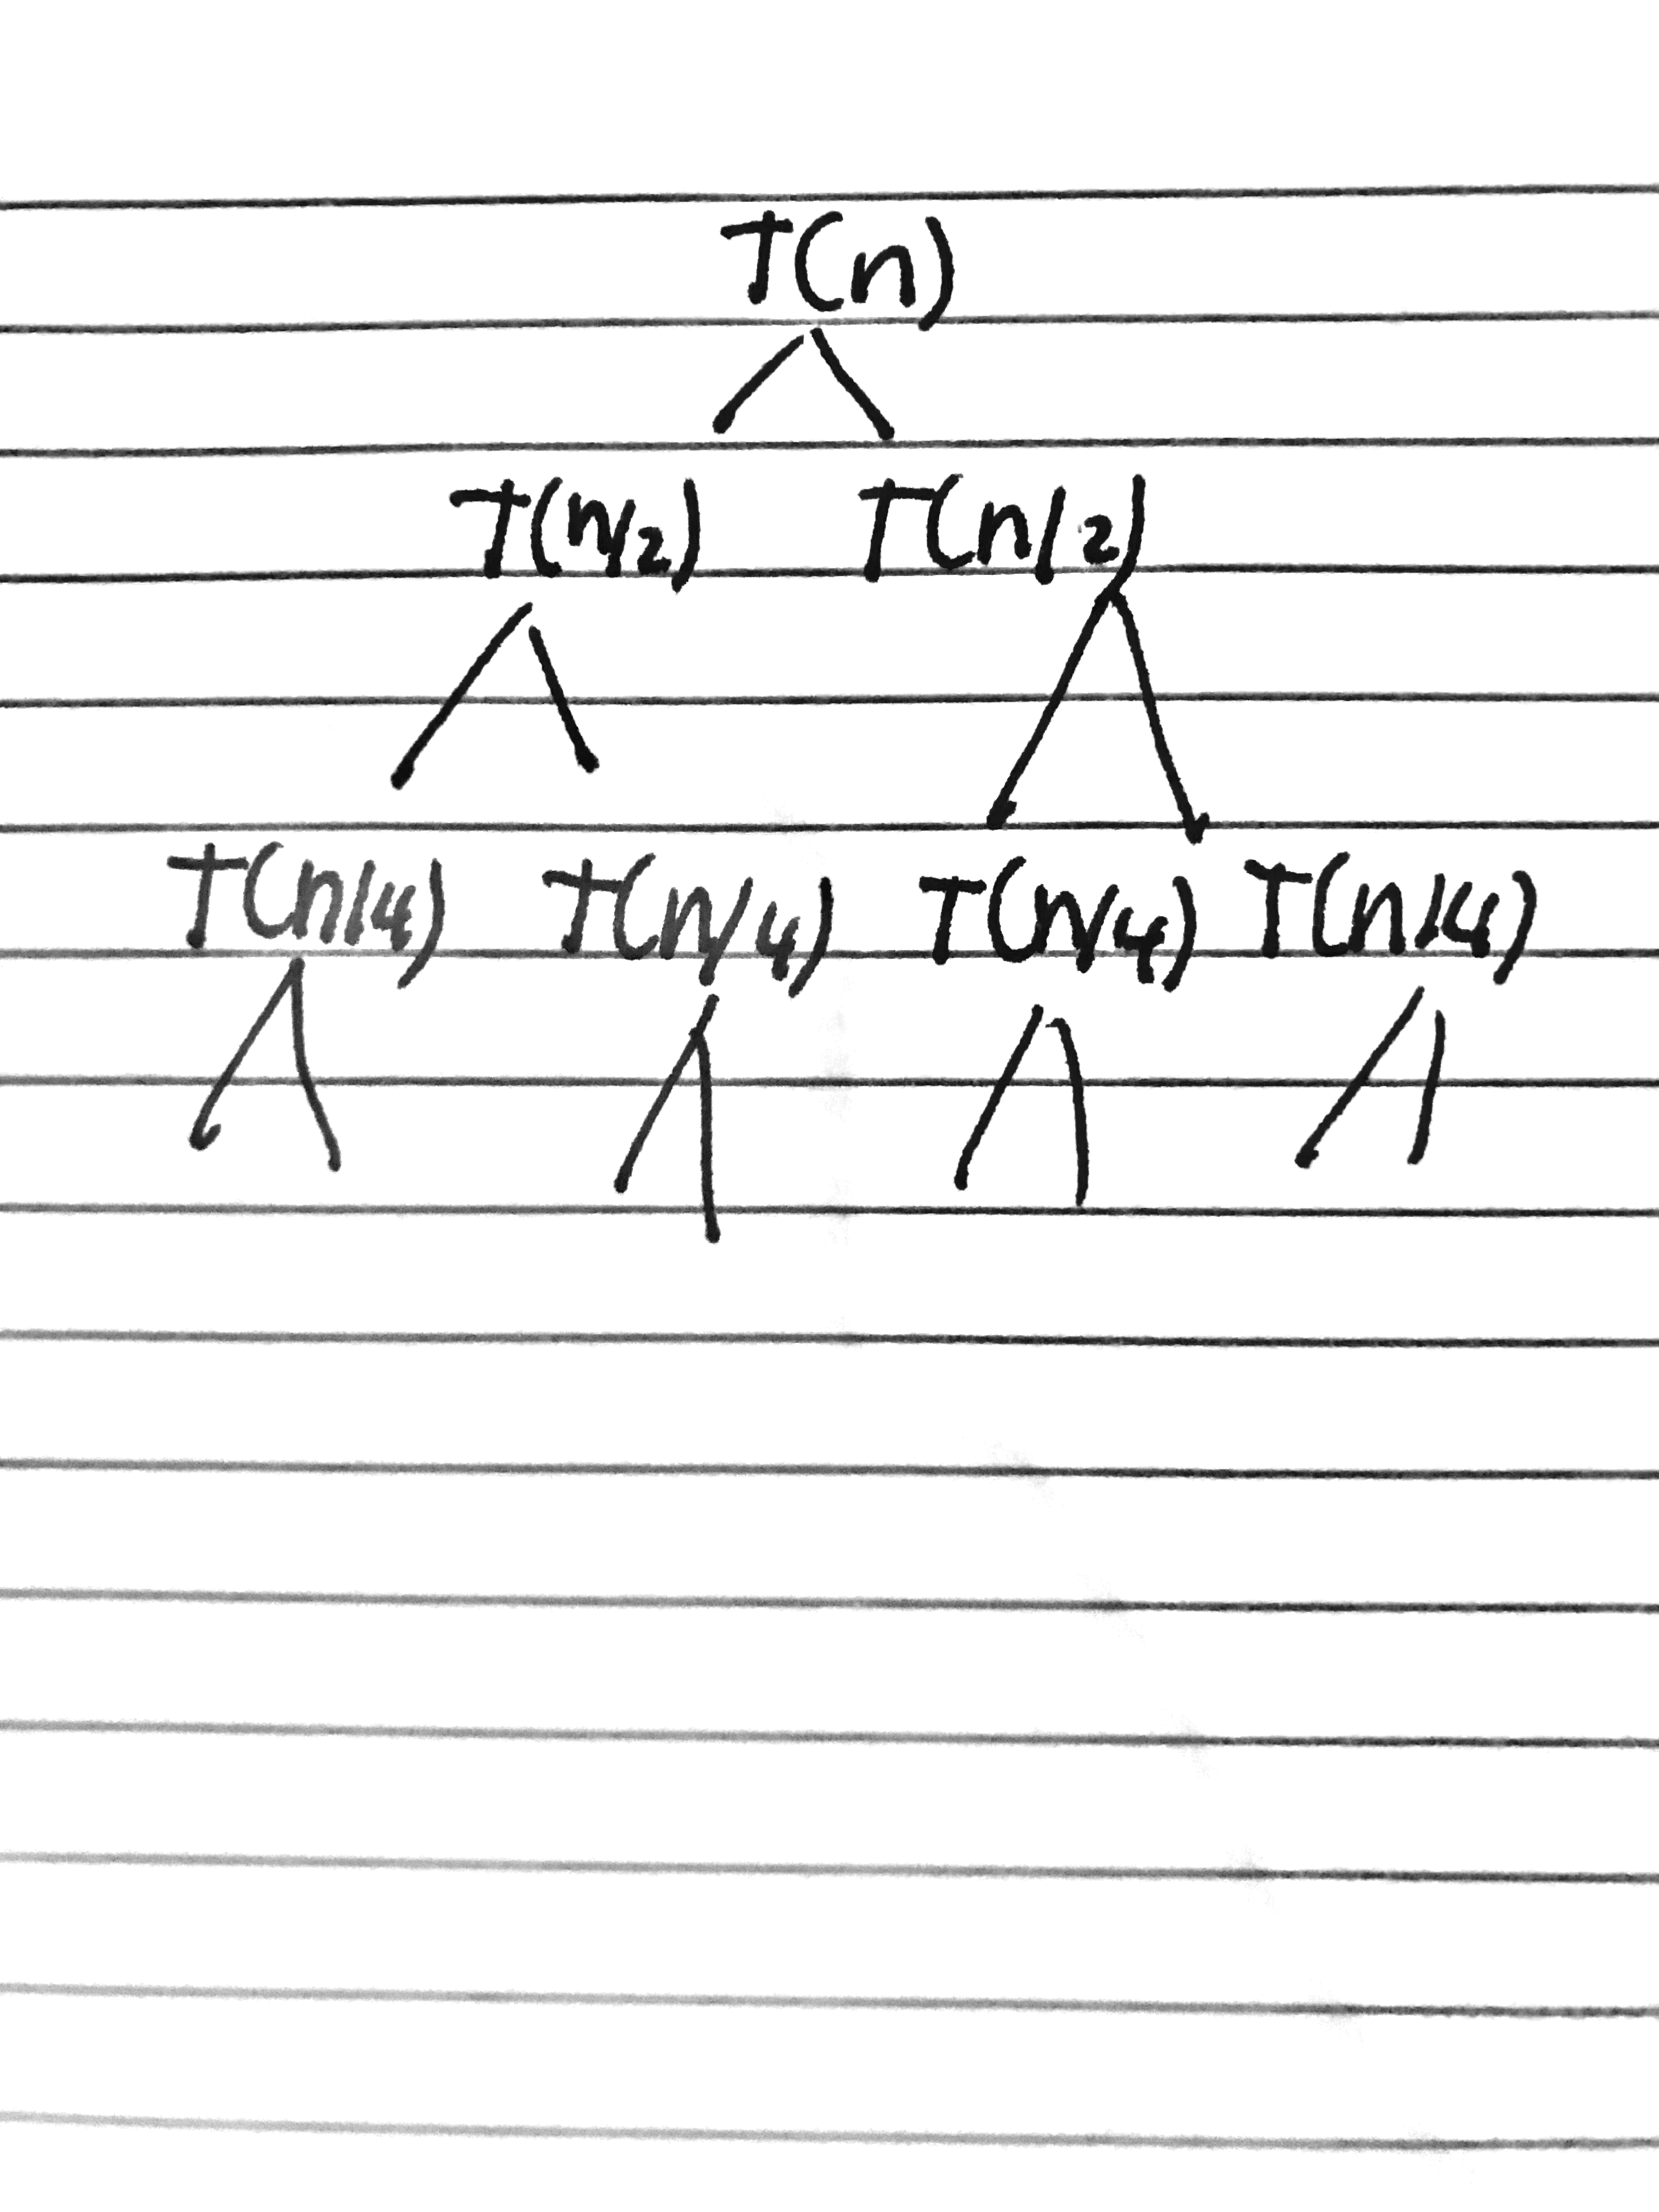
\includegraphics[scale=.05]{./2017-03-271.png}
    \caption{}
    \label{fig:}
  \end{center}
\end{figure}
$$O(\log_2(n)$$

\item (10 points) R-10.17 p. 493\\
For the following statements about red-black trees, provide a justification
for each true statement and a counterexample for each false one.

\begin{enumerate}
\item A subtree of a red-black tree is itself a red-black tree.\\
False. A subtree with a red root must have a black root node

\item The sibling of an external node is either external or it is red. \\
True. If an external node had a black internal brother or sister, the black depth of the external nodes below the black brother or sister would be $h+1$ which is incorrect because all external nodes must have the same black height.

\item There is a unique (2,4) tree associated with a given red-black tree.\\
True.

A node in the red-black tree that contains two red children is represented as a 4-node in 2-4 tree. A node with one red child is represented as a 3-node in the 2-4 tree. A node with 0 red children is represented as a 2-node in the 2-4 tree.


\item There is a unique red-black tree associated with a given (2,4) tree.\\
 False. A 3-node has two different possible ways of being shown in a red-black tree.
 
\end{enumerate}
\item (10 points) R-10.19 p. 493\\
Consider a tree $T$ storing 100,000 entries. What is the worst-case
height of $T$ in the following cases?

\begin{enumerate}
\item $T$ is an AVL tree.
\begin{align*}
h &\le 2\log_2(n+2) \\
h &\approx 33
\end{align*}

\item $T$ is a (2,4) tree.\\
\begin{align*}
h &< \log_{2}(n+1) \\
h &\approx 17
\end{align*}

\item $T$ is a red-black tree.\\
\begin{align*}
h &< 2\log_2(n+1) \\
h &\approx 33
\end{align*}
\item $T$ is a binary search tree.\\
100,000
\end{enumerate}
\item (10 points) R-9.16 p. 418

Draw an example skip list that results from performing the following
series of operations on the skip list shown in Figure 9.12: \texttt{erase(}38\texttt{),
insert(}48,x\texttt{), insert(}24,y\texttt{), erase(}55\texttt{)}.
Record your coin flips, as well.\\ \ \\

Coin flips for $x:$ 4 \\
Coin flips for $5:$ 5

\begin{figure}[h]
  \begin{center}
    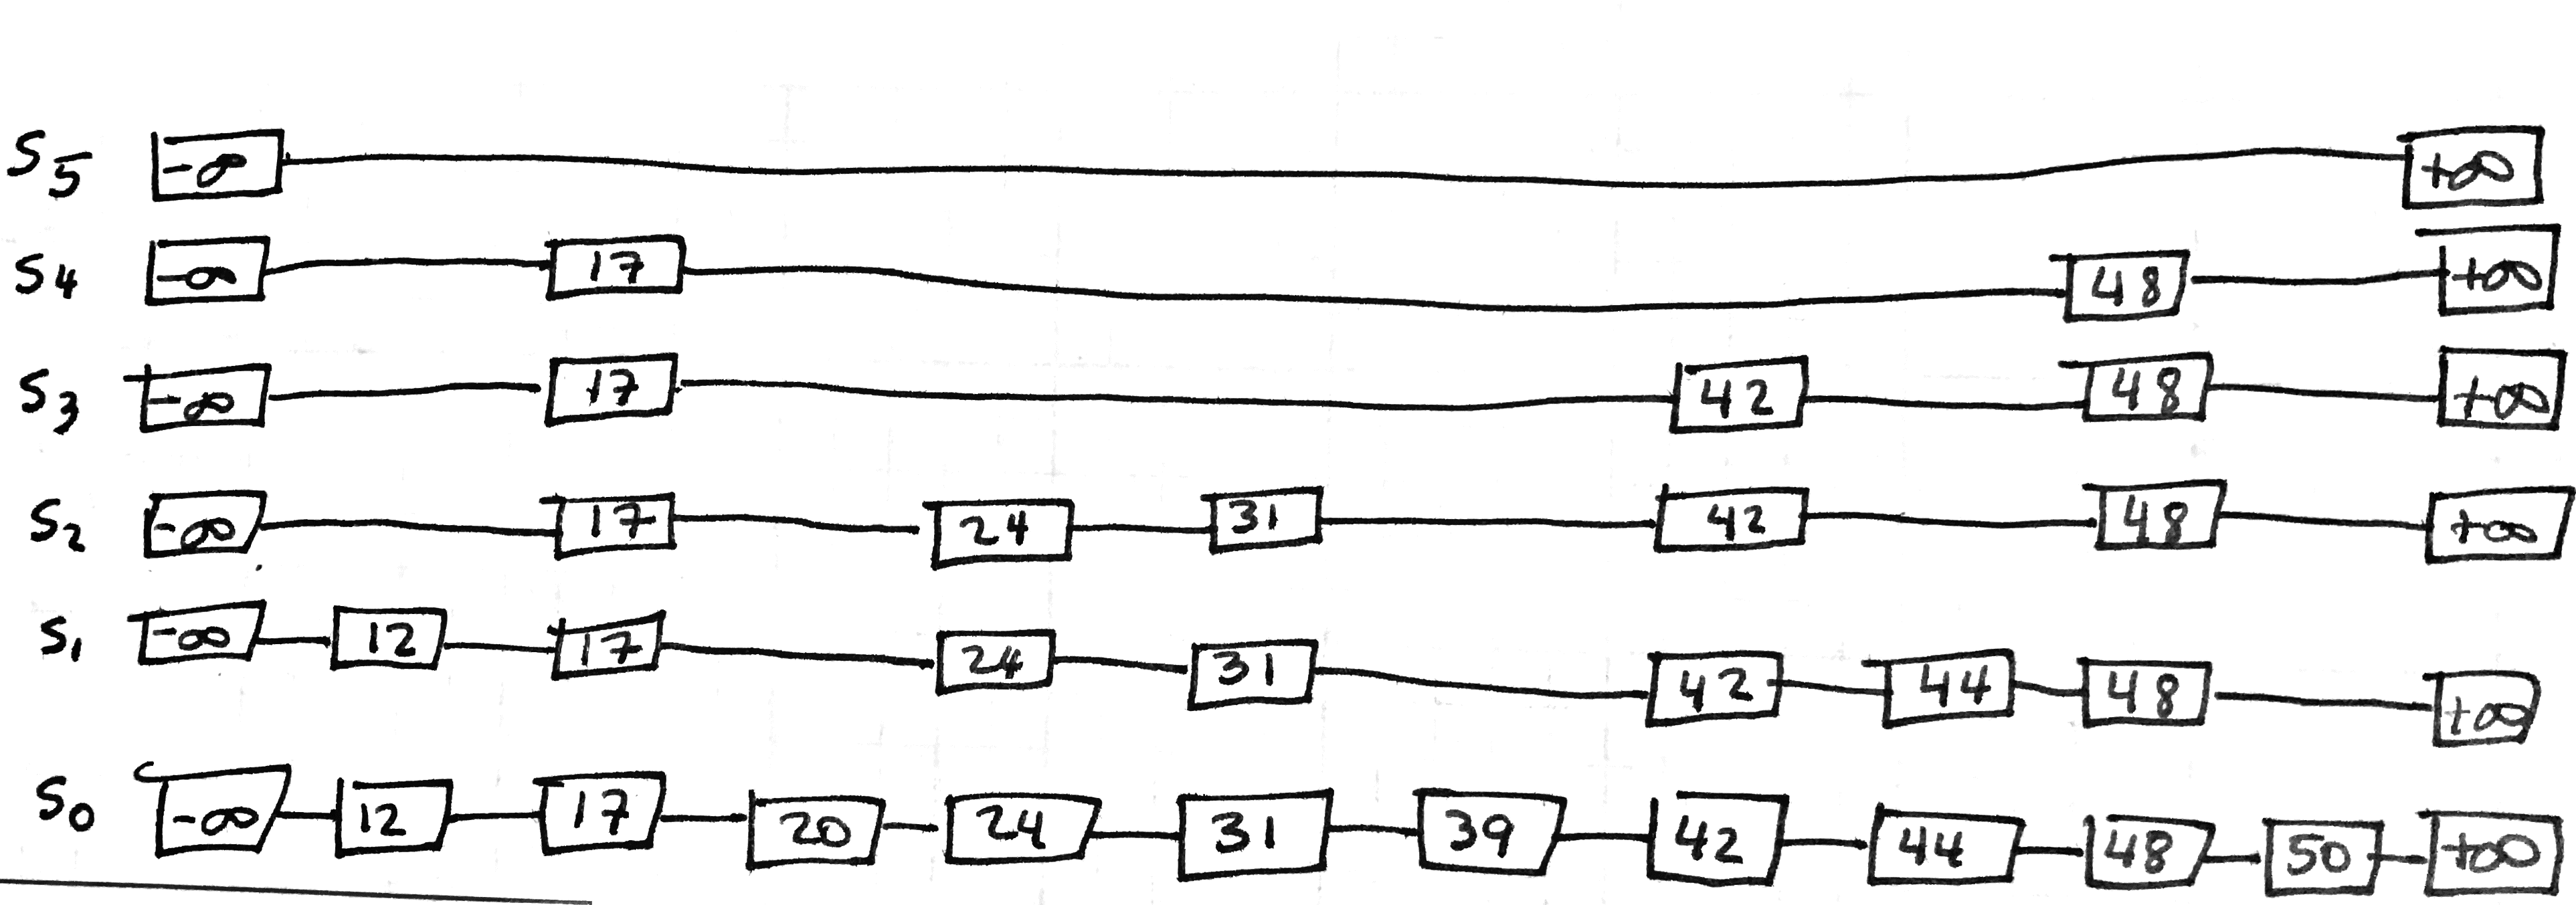
\includegraphics[scale=0.1]{./2017-03-27.png}
    \caption{Skip List}
    \label{fig:}
  \end{center}
\end{figure}
\end{enumerate}

\end{document}
